\resizebox{.97\linewidth}{!}{%
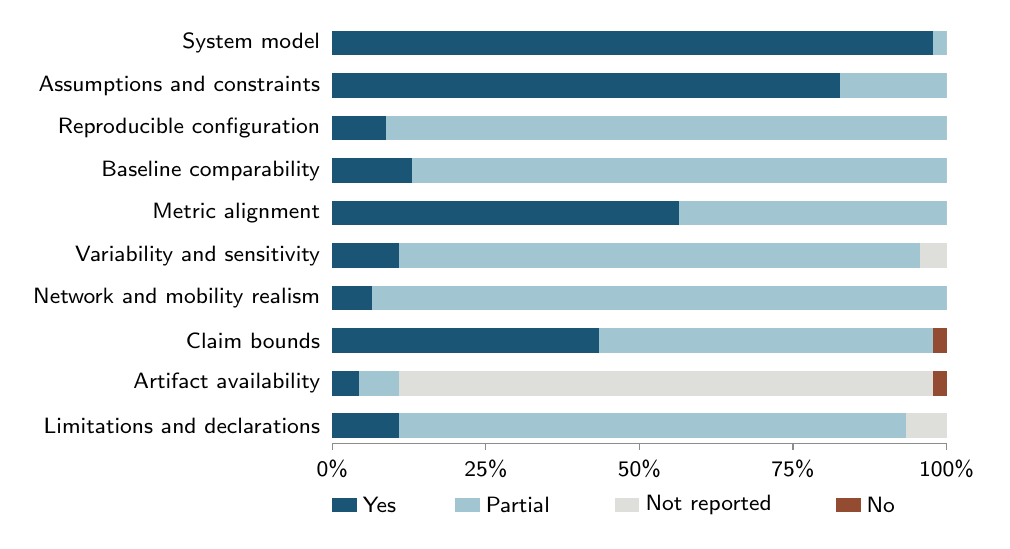
\begin{tikzpicture}[font=\footnotesize\sffamily,y=.54cm,x=.078cm]
\definecolor{appYes}{HTML}{1A5576}
\definecolor{appPartial}{HTML}{A1C5D1}
\definecolor{appNR}{HTML}{DEDEDA}
\definecolor{appNo}{HTML}{934B32}
\newcommand{\appraisalbar}[6]{%
  \node[anchor=east,inner sep=2pt] at (-1,-#1) {#2};
  \pgfmathsetmacro{\yesend}{#3*100/46}
  \pgfmathsetmacro{\partialend}{(#3+#4)*100/46}
  \pgfmathsetmacro{\nrend}{(#3+#4+#5)*100/46}
  \fill[appYes] (0,-#1-.29) rectangle (\yesend,-#1+.29);
  \fill[appPartial] (\yesend,-#1-.29) rectangle (\partialend,-#1+.29);
  \fill[appNR] (\partialend,-#1-.29) rectangle (\nrend,-#1+.29);
  \ifnum#6>0\relax\fill[appNo] (\nrend,-#1-.29) rectangle (100,-#1+.29);\fi
}
\appraisalbar{1}{System model}{45}{1}{0}{0}
\appraisalbar{2}{Assumptions and constraints}{38}{8}{0}{0}
\appraisalbar{3}{Reproducible configuration}{4}{42}{0}{0}
\appraisalbar{4}{Baseline comparability}{6}{40}{0}{0}
\appraisalbar{5}{Metric alignment}{26}{20}{0}{0}
\appraisalbar{6}{Variability and sensitivity}{5}{39}{2}{0}
\appraisalbar{7}{Network and mobility realism}{3}{43}{0}{0}
\appraisalbar{8}{Claim bounds}{20}{25}{0}{1}
\appraisalbar{9}{Artifact availability}{2}{3}{40}{1}
\appraisalbar{10}{Limitations and declarations}{5}{38}{3}{0}

\foreach \tick in {0,25,50,75,100}{
  \draw[black!45] (\tick,-10.42)--(\tick,-10.57);
  \node[anchor=north,inner sep=3pt] at (\tick,-10.60) {\tick\%};
}
\draw[black!45] (0,-10.42)--(100,-10.42);
\foreach \x/\shade/\labeltext in {0/appYes/Yes,20/appPartial/Partial,46/appNR/Not reported,82/appNo/No}{
  \fill[\shade] (\x,-12.03) rectangle (\x+4,-11.70);
  \node[anchor=west,inner sep=2pt] at (\x+4,-11.865) {\labeltext};
}
\end{tikzpicture}}
